\section{Cause and urgency of antibiotic resistance}
The discovery of Penicillin shortly before the Second World War has revolutionized human medicine in the western world by saving the lives of millions of soldiers and civilians. It also made major advances in surgery possible. Ever since then antibiotics play a very important role in our well established health system and we are depending on those drugs in order to fight bacterial infections \cite{worldwar_resistance}.

Because of the positive experience people made during the Second World War with antibiotics, they quickly started to use them in an irresponsible way. This caused a Penicillin resistance within 32 years after it's discovery \cite{worldwar_resistance}. Therefore people realized early on, that extensive use of antibiotics are a thread for the efficiency of those drugs. But the discovery of new antibiotics gave them confidence and the excess of usage of antibiotics went on. Not only were antibiotics continuously prescribed inappropriately they also got introduced into agriculture.
Unfortunately the tendency of irresponsible use of antibiotics increased in the last couple decades. 

For Switzerland the rate of antibiotic consumption divided by the Swiss population stayed the same in recent times, but the absolute consumption increased. This is because more people were getting treated in hospitals \cite{swiss_hospitals} but the general population of Switzerland increased too.     
Furthermore antibiotic resistance is a global issue. Compared to other countries Switzerland is on the lower end when it comes to antibiotic doses per 1000 people \cite{swiss_hospitals}. Additionally other countries also have a very high use of antibiotics in agriculture, exposing a lot of bacteria to a lot of antibiotics, giving the bacteria an ideal environment to evolve and gains resistance. Since traveling started to get a lot more popular with long-distance traveling in particular, there is a globally ongoing exchange of resistant pathogens. This increases the difficulties of managing resistant pathogens because fighting the antibiotic resistance crisis locally is not going to help much because of this global exchange.  

In Switzerland the biggest challenge with resistant pathogens is ongnoind in hospitals. In such institutions, obviously a lot of people need treatment against bacterial infections, leading to an accumulation of pathogens but also to very locally applied high doses of antibiotics.
Therefor Swiss hospitals turned into hot-spots of antibiotic resistant pathogens.
Unfortunately a lot of people within the hospitals are weakened by diseases causing a worse functional immune system and therefore such patients are a lot more vulnerable to infections with antibiotic resistant bacteria.
This combination of an increasingly number of antibiotic resistant bacteria and very vulnerable patients lead to a very urgent problem in modern medicine causing about 300 deaths, patients having to spend more time in hospitals and high costs \cite{anresis}.

\subsection{An overview of antibiotic resistant pathogens in Swiss hospitals}
Mainly four strains which cause problems in treatment with antibiotics are present in Swiss hospitals:\\
\begin{figure}[H]
	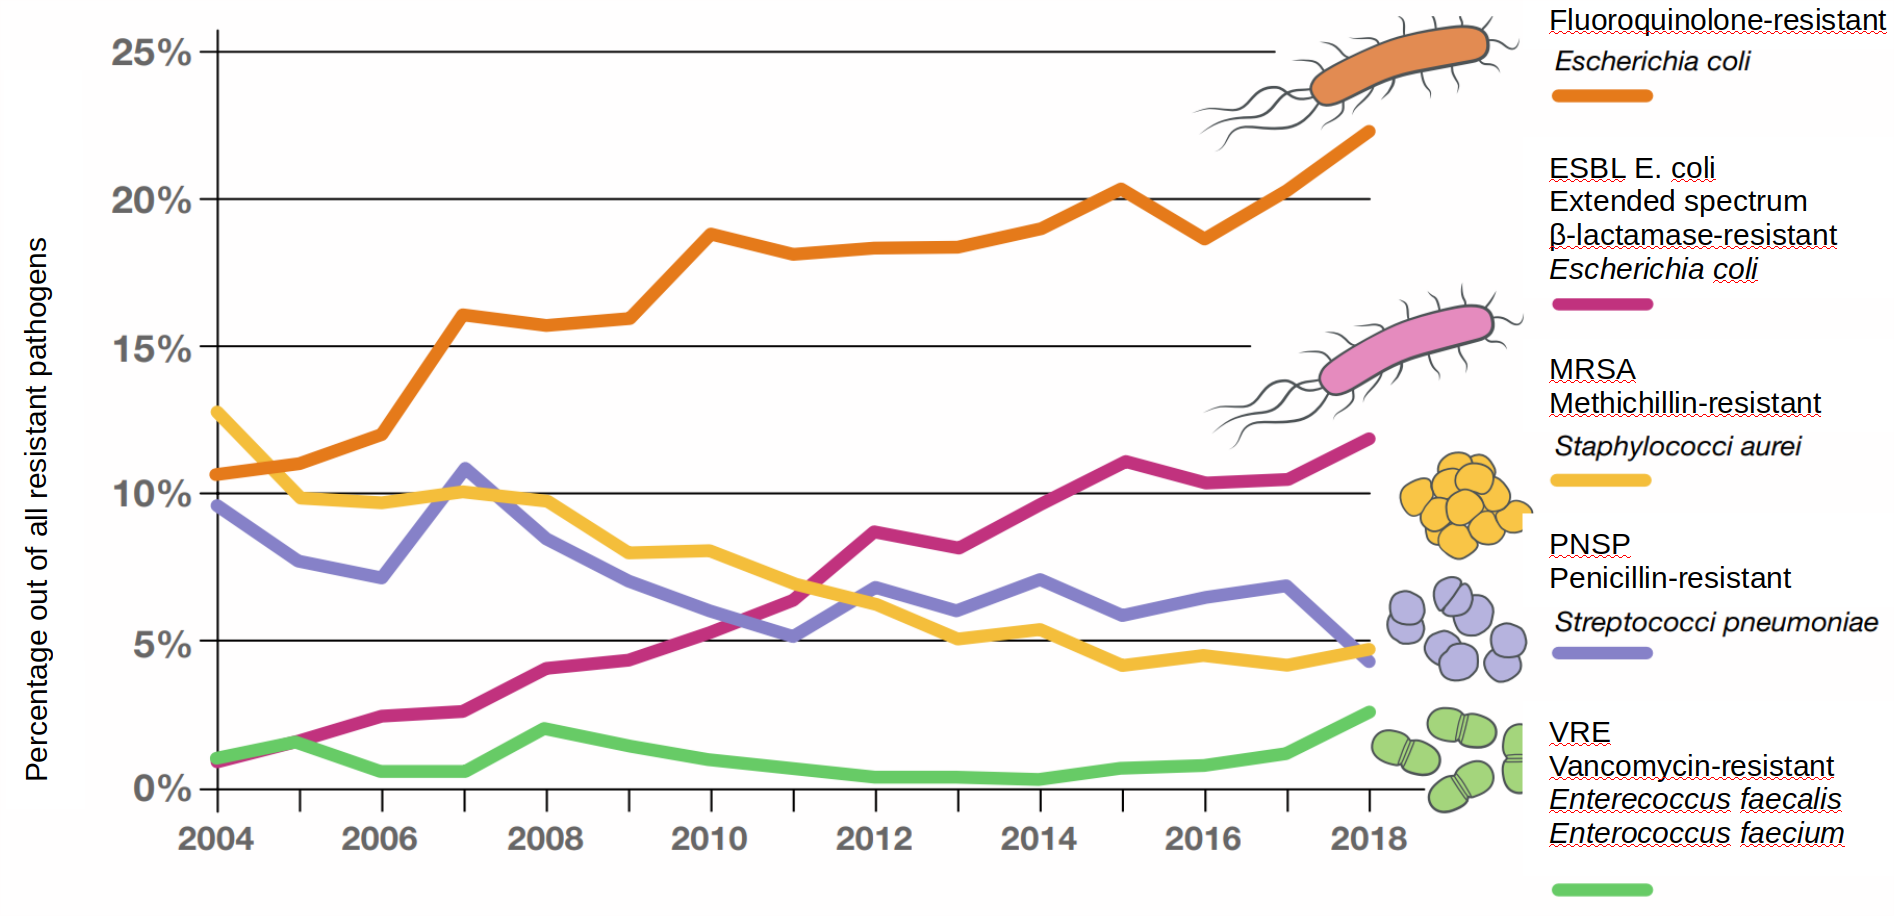
\includegraphics[scale=0.2]{pathogens_overview.png}
	\caption{Development of popularity of antibiotic resistant pathogens.
	\cite{swiss_hospitals_pathogens}}
	\label{figure:pathogen_dvelopment}
\end{figure}
\textbf{Staphylococcus aureus} usually doesn't cause any diseases in healthy people. But if someone's immune system is weakened they can cause skin and bone inflammations. Staphylococcus aureus is causing the most infections for surgical wounds.

\textbf{Streptococcus pneumoniae} are present normally in the nose and throat of everyone. For weak people this strain can turn into a pathogen causing several thousands blood infections and pulmonary infections per year. 

\textbf{Klebsiella pneumoniae} is one of the biggest problems for swiss hospitals. They can cause severe pulomnary infections and blood infections which can be very dangerous for newborns \cite{swiss_hospitals_pathogens}.

\textbf{Escherichia coli (E. coli)} belongs to the enterobacteriaceae and is present in every intestine where they are not dangerous. However they are able to cause infections when present in other parts of the body leading mainly to infections of the urinary tract but also in the brain of new borns. 

Mainly E. coli and Staphylococcus aurei have been increasingly reported in context of antibiotic resistant infections over the last 15 years as visible in Figer \ref{figure:pathogen_dvelopment}. On the other hand antibiotic resistant infections with Streptococci pneumoniase and Entereococcus remained more or less the same or decreased slightly.
It is noteworthy how fast the numbers of infections with extended spectrum \textbeta-lactamase (ESBL) producing E. coli increased within 15 years. In 2004 they only made up for about 1 \% of all antibiotic resistant pathogens, 2018 they are already at 12 \% with an uprising tendency. This is causing a lot of concerns and problems in hospitals because as the name already implies, those pathogens are able to hydrolyze an extended spectrum of \textbeta-lactams forcing doctors to prescribe antibiotics of last resort.

Because of this threat coming from ESBL E. coli I dedicate this thesis entirely to this pathogen. Unfortunately it is not completely understood yet, how those enterobacteriaceae are able to produce such a strong resistance against many \textbeta-lactams. My goal is to generally get a better understanding of genes involved in the evolution of resistance and potentially identify new genes which could play an important role in the resistant mechanisms. 

\section{Extended-spectrum -lactamases (ESBL) E. Coli}
Extended \textbeta-lactamases (ESBLs) are certain \textbeta-lactamases which are able to hydrolyze extended-spectrum cephalosporins with an oxyimino side chain. Such cephalosporins are aztronam, cefotxamie or ceftazidime for example \cite{esbl_introduction}. 
Some ESBLs arose by mutations in genes for common plasmid-mediated \textbeta-lactamases such as TEM and SHV enyzmes. Those ancestors were able to hydrolyze regular \textbeta-lactamases but were susceptible to cephalosporins \cite{esbl_introduction_emerg}. 
There are also new families of ESBLs, such as CTX-M and OXA \cite{ctx-m} which evolved independently from the ESBLs which have their origin in the TEM and SHV enzymes. 

Those newly formed \textbeta-lactamases are increasingly reported as reasons for resistance, in contrast to the other \textbeta-lactamases related to TEM and SHV which generally decrease in popularity.
CTX-M is a group of \textbeta-lactamases with CTX-M-1 being the most popular one. There are many more characterized CTX-M enzymes, most of them differ by just one amino acid. With a sequence identity compared to TEM and SHV of only 40 \% \cite{ctx-m}, it's assumed that they evolved from a different precursor. It's assumend that they evolved from the \textbeta-lactamase precursor AmpC from Klyzvera ascorbata  \cite{ctx-m}. Even though the first CTX-M-1 was isolated in Germany, it's mostly popular in eastern Europe, South America and Japan.
The OXA family was originally created as a phenotypic rather than a genotypic group, based on a specific hydrolysis profile. Therefor the sequence identity compared to other members of this family is only about 20 \%. It's name comes from the ability to efficiently hydrolyze oxacillin \cite{ctx-m}.
   
ESBL E. Coli can be detected using isothermal amplification, PCR or microarrays. Since ESBL E. coli are able to hydrolyze cephalosporine, doctors prescribed carbapenems or potent \textbeta-lactam-\textbeta-lcatamase inhibitor (BLBLI) combinations, when ESBLs were detected with the methods above. However it turned out that some E. coli expressing ESBLs are actually susceptible to oxymino-cephalosporins \cite{esbl_introduction}. This showed, that the prescription of antibiotics of last resort because a pathogen tested positive for ESBLs was unnecessary in some cases. Since antibiotics of last resorts are incredibly valuable it's in the interest of everyone to only use them if urgently necessary. Irresponsible prescription on the other hand will cause further resistance in a rather short time scale. 
Since a simple presence/absence check of ESBLs is not giving the necessary information in order to decide whether antibiotics of last resort are needed, those tests are now getting ignored as ordered by the EUCAST \cite{eucast}. It's recommended to test susceptibility in vitro which takes about 48 hours which is a lot longer than genetically testing. For patients in acute stages of inflammation 48 hours is too long, forcing doctors to still prescribe antibiotics of last resort even when it's not known if the pathogen would be susceptible to common cephalosporins. 
Since some ESBL producing E. coli are genetically resistant but phenotypically susceptible there must be other mechanisms involved in the resistance path next to a simple presence or absence of \textbeta-lactamases. 

Other ways to protect the pathogen from the drug could be a less permeable outer membrane of the pathogen. It's also possible that resistant pathogens have a higher efflux activity, leading to an active transport of the drug, out of the cell. In combination this would mean a lower influx and a higher efflux, which would work in favor of the pathogen. Furthermore another option would be that the copy number of genes coding for ESBLs varies within ESBL E. coli, deciding over resistance or susceptibility. 

With this thesis I try to get a better understanding on which strategies are involved in resistant ESBL E. coli. I'm doing this by combining two different approaches, one being a bioinformatic analysis with ESBL E. coli isolates from patients, the other being a more experimental approach.\\ 


For the first part of this project I try to identify changes in the genome from ESBL E. coli samples isolated from our collaborator Adrian Egli at the University hospital Basel. Those samples made a transformation from being susceptible to \textbeta-lactams to resistant, or they lost their ability to hydrolyze cephalosporins. 

For the experimental part of this project I assemble a system called morbidostat which allows to continuously monitor E. coli cultures and automatically putting them under antibiotic pressure, by injecting appropriate drug doses. This causes evolution and selection which can be observed in real time. Along this process samples can be taken and analyzed with a similar pipeline as for the clinical isolates.

\section{Longitudinally collected ESBL E. coli isolates from patients from the University hospital Basel}
Our collaborator Adrian Egli, head of the clinical microbiology from the University hospital Basel, collected Isolates of patients who were infected with ESBL E. coli. His group determined the MIC of the cephalosporines cefepime and ceftazidime for every collected isolate  and short-read sequenced thme on a MiSeq Illumina system.
This resulted in a data collection with multiple isolates per patient, where a change of MIC for cefepime and ceftazidime was visibile over time caused by gained or lost resistance. 
The principle of this analysis is, to build a very accurate reference genome for each patient based on the isolate with the lowest MIC for the tested cephalosporines. The isolate with the lowest MIC is also called wild-type. Then the other isolates with a higher MIC can be compared to this reference genome and changes can be identified. 

This can be done by mapping the Illumina sequencing data from the resistant isolates to the reference genome from the wild-type. 
This makes possible to identify single-nucleotide polymorph positions (SNPs) in the genome of the resistant samples. Because tools for annotating genomes are available, it's possible to filter for SNPs which are affecting known genes or promoter regions. Based on this information it should be possible to get more insights in the evolution of resistance. 

Since this analysis is depending on very accurately assembled reference genomes we additionally long-read sequenced isolates of interest with Oxford Nanopore Technologies. Illumina returns very accurate short reads (75 bp) but because the reads are so short it's computationally not possible to assemble those reads structurally correct. On the other hand reads produced with Nanopore Technologies are extremely long (up to 200 kbp) but quite inaccurate based on issues with repetitive nucleotide sequences. However both techniques combined together return an assembly with a nucleotide error rate from Illumina but also with a high accuracy in terms of structural information.  
This strategy of combining short- and long-reads is also known as hybrid assembly. 


\section{Building a morbidostat} 
Since we wanted to experimentally force susceptible ESBL E. coli to gain resistance over a rather short time period, we had to come up with a system which allows to constantly put E. coli under antibiotic pressure. Such constant antibiotic pressure forces evolution of resistance and for selection of mutants. Such a system has already been invented by Toprak et al. \cite{morb_toprak} which he called morbidostat, an automated continuous culture device. Based on the invention of Toprak we rebuild a morbidostat with small modifications which should improve the handling and mainly make it a lot more compact which is important since we want to use the morbidostat in a space limiting hypoxi-station. With our version of the morbidostat 15 cultures can be grown independently in vials. Thereby the growth of each culture is monitored by measuring and saving the optical density (OD). Based on the growth an appropriate dose of antibiotics is injected into the culture leading to an inhibition of the growth without entirely killing ever colony forming unit. The appropriate dose of antibiotics is achieved by mixing different drug concentrations using computer controllable pumps which are also injecting the drug into the vials.
The morbidostat allows to study drug resistance evolution in real-time, while having an idea of the progress of evolution in resistance. Since the goal is to identify changes in the genome while the strain gains resistance, samples have to be collected every other day, in order that the DNA can be isolated and sequenced.

In the morbidostat, bacteria are grown in a fixed volume. The process of suppressing the growth with antibiotics is divided into cycles which are constantly getting executed. One cycle has following tasks and commands:
\begin{itemize}
	\item Measuring the OD every several seconds over a defined cycle time \textDelta t 
	\item Calculating growth rate at the end of the cycle based on the previously collected ODs
	\item Based on growth, injection of appropriate dose of drug, as calculated by a feedback algorithm
	\item Getting rid off volume which exceeds fixed culture volume
\end{itemize}

\begin{figure}
	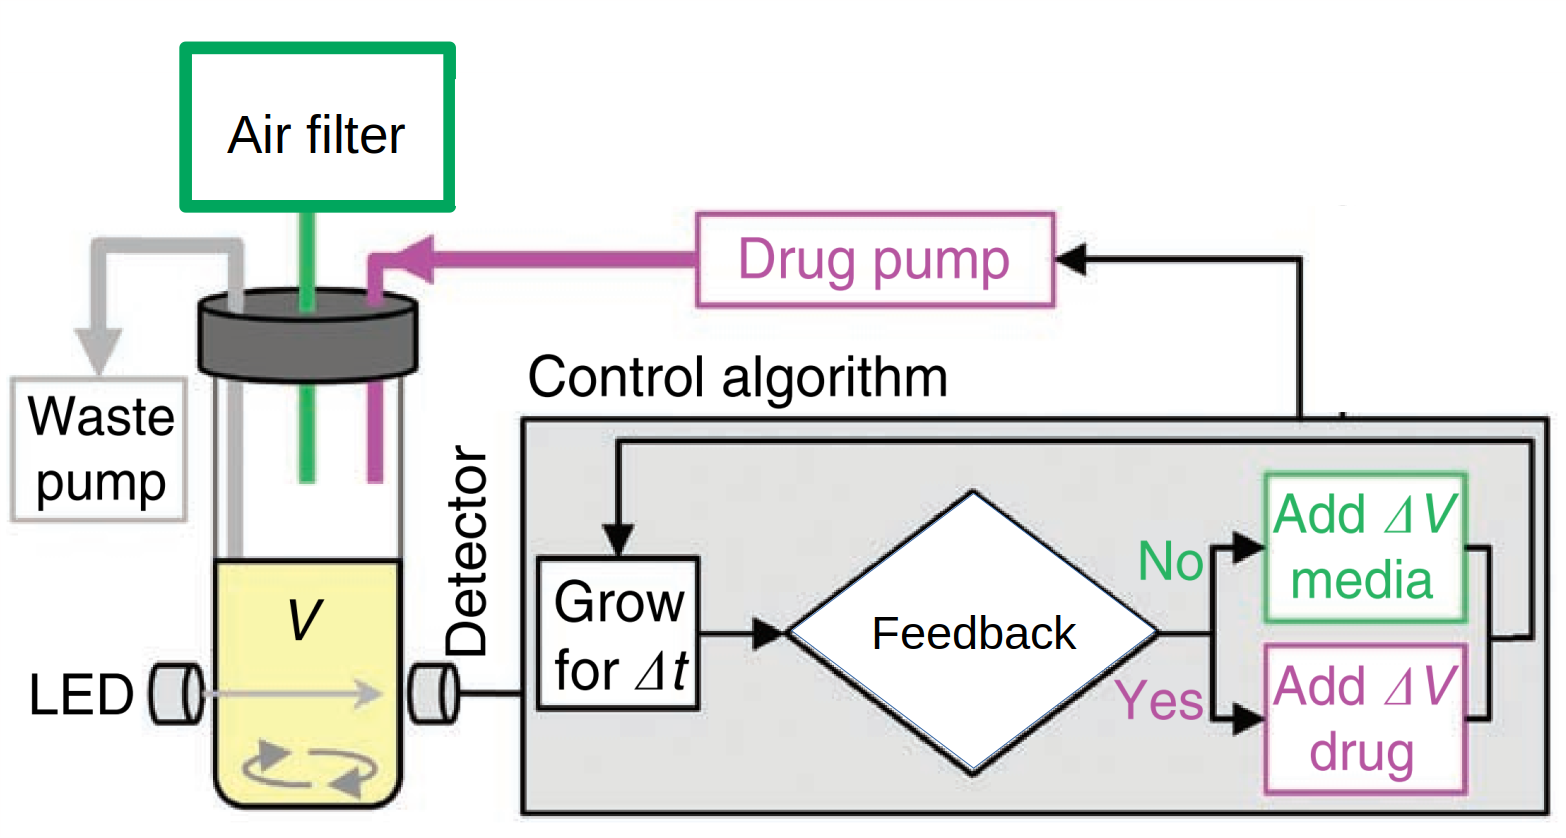
\includegraphics[scale=0.1]{vial_diagram.png}
	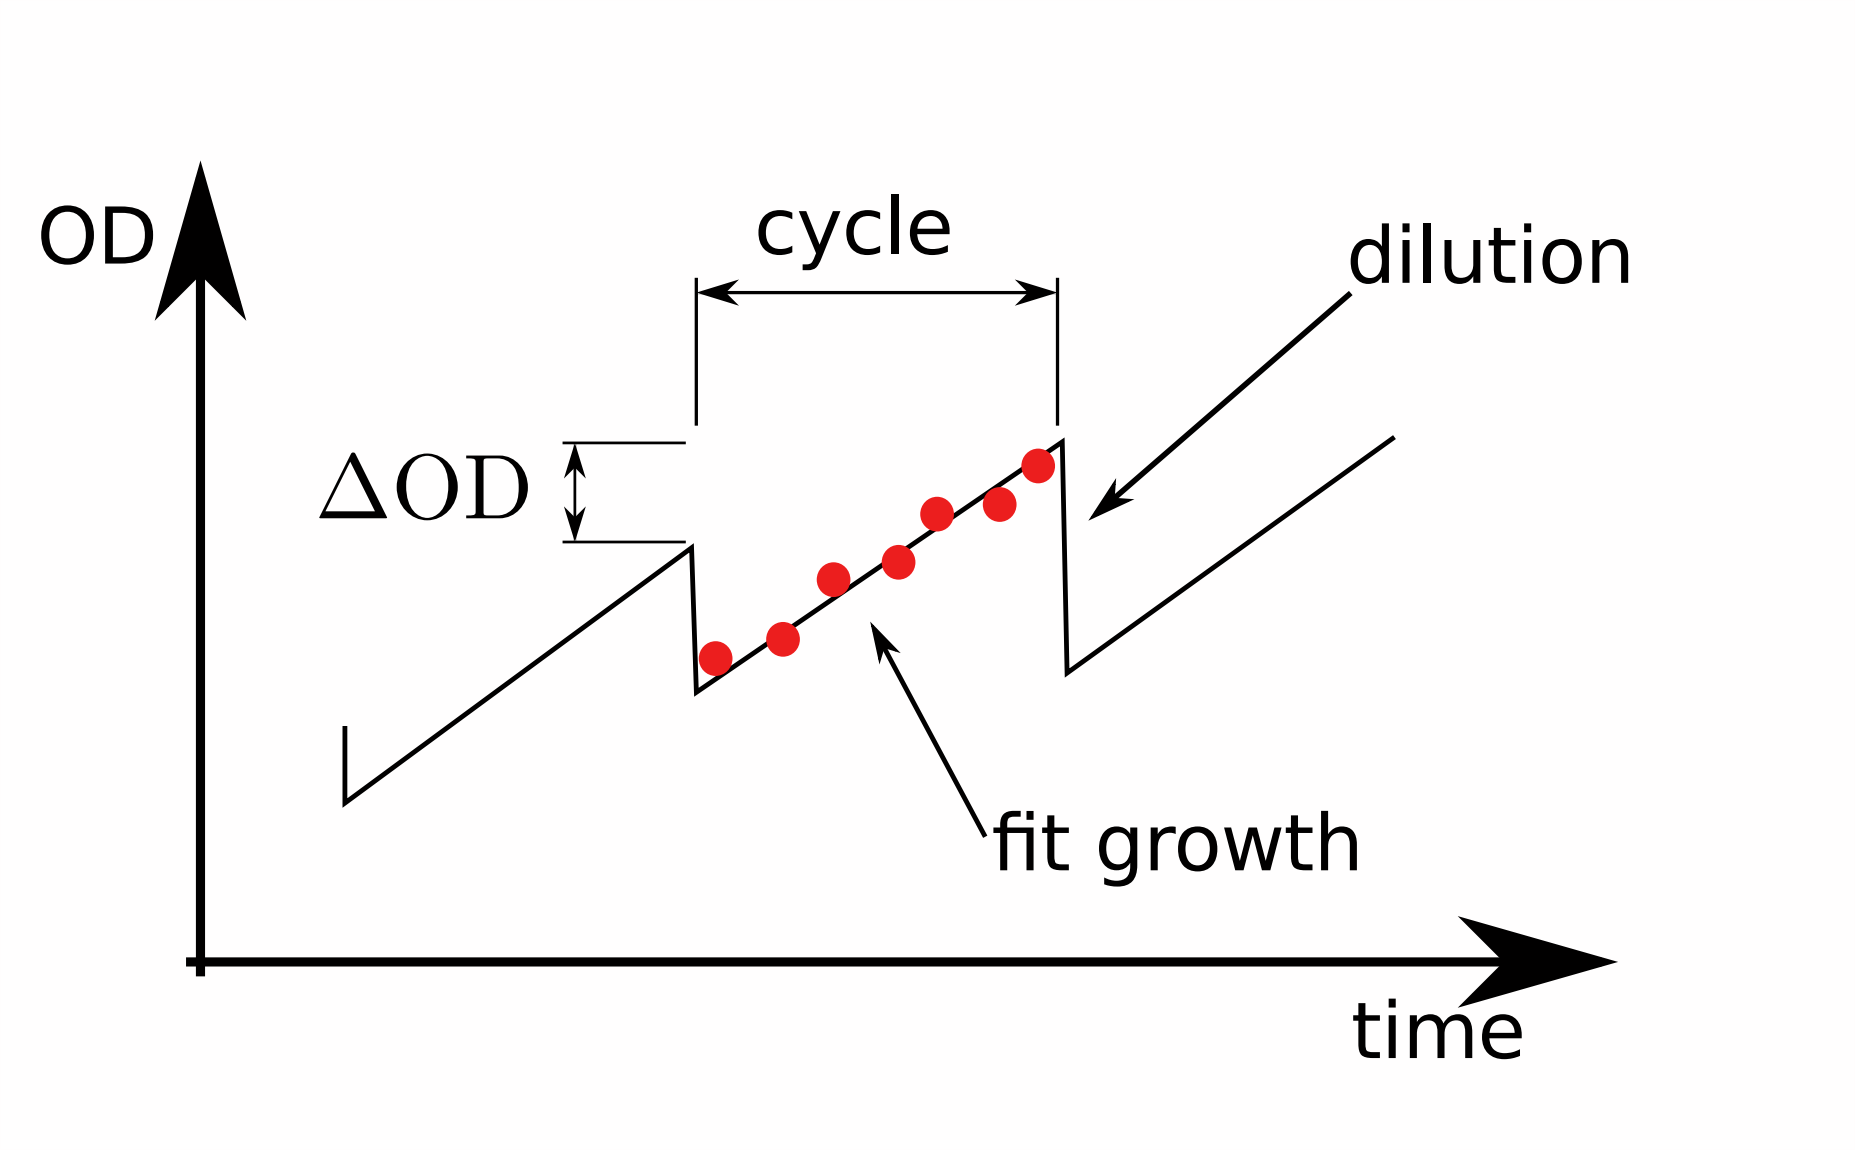
\includegraphics[scale=0.07]{growth_diagram.png}
	\caption{Based on the growth a feedback algorithm decides whether and how much drug is getting injected}
	\label{figure:vial_setup}
\end{figure}

\subsection{Drugs of interest and bacteria of choice for the experiments}
\subsubsection{Choice of ESBL bacteria for the morbidostat experiments}
Initially the idea was to cultivate the wild-type isolates from the sample collection provided from Adrian Egli and which were also used for the bioinformatics analysis. This would have been nice, because it would have allowed to compare evolution taking place under physiological conditions and forced evolution by the morbidostat. 
Even though the morbidostat is run inside an air tight hypoxystation within a bio safety lab 2, it was decided that it's to risky to do the experiments with the ESBL E. coli coming from the hospital. Instead we decided to clone the \textbeta-lactamase sequences from the wild type samples into a plasmid transformed into K12 E. coli which is not able to infect humans.

Concerning the drugs, cefepime and cefatzidime were chosen, since those drugs were also used for the treatment of the ESBL E. coli from the sample collection from the hospital.\\
Both caphalosporines are effectively bactrocidal against gram-negative bacteria and act by inhibiting the synthesis of the peptidogylcan layer of gram negative bacterial cell walls. cefepime is reagrded as a 4th-generation cephalosporin and was developed with ceftazidime as a foundation. Reistance against ceftazidime often emerged due to hydrolysis by the AmpC \textbeta-lactamase. Cefepime was designed with a change in its 3' side chain, which should protect the drug from hydrolysis \cite{cefepime}.  








 






